\documentclass{article}
\usepackage{graphicx}
\usepackage[margin=2cm]{geometry}
\usepackage[none]{hyphenat}

\def\code#1{\texttt{#1}}

\setlength{\parindent}{0pt}

\begin{document}

\begin{titlepage}
    \centering
    
    \Huge \textbf{Regenboogboom}
    \vspace{1cm}
    
    \Large Noah Van Steenbrugge
    
    \large $2^{de}$ Bachelor Informatica
    \vspace{5cm}

    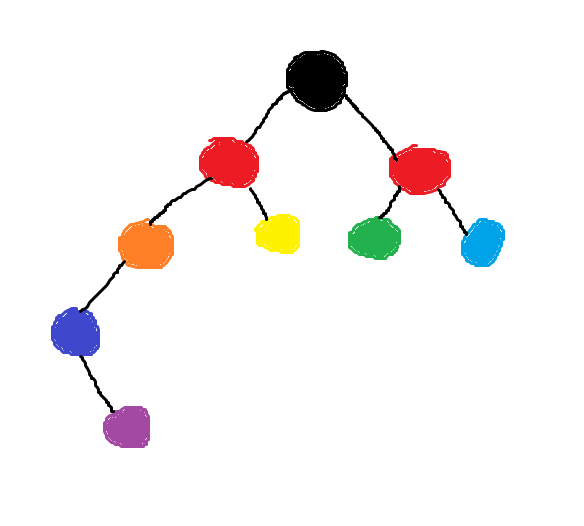
\includegraphics[width=0.5\textwidth]{regenboogboom.png}
\end{titlepage}

\newpage
\setcounter{page}{1}

\section*{\centering DEEL I: theorievragen}
\vspace{1cm}

\Large 1. Rood-zwart boom $T$ met $n$ sleutels en $m$ toppen
\vspace{0.5cm}

\Large (a) kleinst aantal rode toppen in $m$
\vspace{0.3cm}

\large
Dit kunnen we bepalen met een paar recursieve berekeningen

Voor $n < 2$ hebben we 0

Voor $n \geq 2$ bepalen we de toppen voor de linker- en rechterrecursie en noemen deze $n_l$ en $n_r$

We starten met $n_l = 2^{\lfloor \log(n+1) \rfloor} - 1$ en $n_r = 2^{\lfloor \log(n+1) \rfloor - 1} - 1$

Hierdoor hebben we in de deelbomen van de kinderen exact genoeg toppen om een complete boom te maken voor $d_l = \lfloor \log(n+1) \rfloor - 1$ links en $d_r = \lfloor \log(n+1) \rfloor - 2$ rechts

Dus nu hebben we links teveel toppen, rechts te weinig toppen of perfect genoeg toppen

Dit veranderen we makkelijk met $diff = n - 1 - n_l - n_r$:

Als $diff < 0$, hebben we er links teveel en trekken we $| diff |$ af van $n_l$

Als $diff = 0$, zitten we goed

Als $diff > 0$, hebben we er rechts te weinig en tellen we $diff$ op bij $n_r$

Maar in de gevallen waarbij $diff \geq 0$ hebben we in de linkerdeelboom $d_l + 1$ zwarte toppen in een pad van de wortel naar een NULL-pointer

Terwijl we in de rechterdeelboom $d_r + 1$ in zo'n pad hebben en $d_r = d_l + 1$

Dit lossen we makkelijk op door de wortel van de linkerdeelboom rood te kleuren

Dus ons kleinst aantal rode toppen voor $n$ is het kleinst aantal toppen voor $n_l$ en dat voor $n_r$ plus 1 als $n - 1 - n_l - n_r \geq 0$

\vspace{0.2cm}

Hiermee heb ik dit eigenlijk ook al bewezen met inductie

IB: $n < 2$ levert het kleinst aantal op (logisch)

IH: stel het geldt voor $n_l$ en $n_r$

IS: voor het aantal rode toppen voor $n \geq 2$ is het enige verschil met $n_l$ en $n_r$ de correctieterm

Maar deze kunnen we niet vermijden, aangezien we anders geen rood-zwart boom meer hebben

\normalsize IB, IH en IS staan resp. voor inductiebasis, -hypothese en -stap 

\vspace{0.5cm}

\Large (b) algoritme om $T$ op te bouwen met zo weinig mogelijk rode toppen
\vspace{0.3cm}

\large
Dit algoritme zal verschillen met de recursieve berekeningen van de vorige vraag, omdat ik wil aantonen dat er meer mogelijkheden zijn om hetzelfde resultaat te krijgen (er werd uitvoerig getest of het aantal rode toppen mooi overeenkomt met de recursieve methode)

\vspace{0.2cm}

We starten met het opvragen van de sleutels in gesorteerde volgorde

Dan zullen we de grootst mogelijke compleet binaire boom opbouwen met enkel zwarte toppen

Hierna voegen we de overgebleven sleutels toe als rode toppen van links naar rechts (het is belangrijk dat we de sleutels voor de compleet binaire boom zodanig kozen, zodat dit mooi van links naar rechts kan)

Maar indien we op deze manier de $i^{de}$ sleutel toevoegen, waarbij $i$ even is, zullen we de ouder van deze sleutel rood kleuren en de kinderen hiervan zwart

Indien $i / 2$ weer even is, zullen we de ouder van de ouder rood kleuren en de kinderen hiervan weer zwart en zo doen we dit in totaal $k$ keer tot $i / 2^{k+1}$ niet meer even is

Nu hebben we onze boom opgebouwd met het minimum aantal rode toppen

\newpage

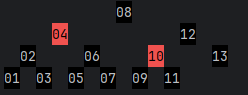
\includegraphics[width=0.5\textwidth]{redblack_rebuild_13.png}

\vspace{0.2cm}

Hier een voorbeeld van de rebuild voor n = 13

\vspace{0.5cm}

\Large (c) tijdscomplexiteit
\vspace{0.3cm}

\large
Het opvragen van de sleutels in gesorteerde volgorde kan in $O(n)$, door deze recursief te doorlopen (zie mijn implementatie voor \code{values()} in DEEL II)

Dan doen we een aantal berekeningen in $O(1)$ om te zien wat de diepte wordt van onze grootst mogelijke compleet binaire boom

Hierna lopen we over de sleutels en kiezen we degene uit die we zullen gebruiken voor de opbouw van de compleet binaire boom in $O(n)$

Uiteindelijk bouwen we onze compleet binaire boom recursief op in $O(n)$

Het toevoegen van de resterende sleutels kan in $O(n)$, dankzij een bijgehouden lijst, waarbij we de ouders in $O(1)$ kunnen bepalen (en ook de ouder van de ouder voor het geval dat $i / 2$ even is enz.)

Dus is onze tijdscomplexiteit $O(n)$

\vspace{0.5cm}

\Large (d) tijdscomplexiteit voor een reeks van $b$ bewerkingen op een initiëel lege boom
\vspace{0.3cm}

\large
bovengrens toevoegbewerking:

Het maximaal aantal toppen in de boom is $b$, dus een bovengrens is $b * O(\log(b)) = O(b * \log (b))$, aangezien onze toevoegbewerking een tijdscomplexiteit heeft van $O(\log(n))$, met $n$ = aantal toppen

\vspace{0.2cm}

bovengrens opzoekbewerking:

Het maximaal aantal toppen in de boom is $b$, dus een bovengrens is $b * O(\log(b)) = O(b * \log (b))$, aangezien onze opzoekbewerking een tijdscomplexiteit heeft van $O(\log(n))$, met $n$ = aantal toppen

\vspace{0.2cm}

bovengrens verwijderbewerking:

Bij een verwijderbewerking is er meer werk, want de tijdscomplexiteit voor een enkele operatie is $O(n)$ (indien rebuild zich voordoet)

Maar we kunnen bewijzen dat een bovengrens voor $b$ verwijderbewerkingen $O(b * \log(b))$ is:

Een verwijderbewerking heeft tijdscomplexiteit $O(\log(n))$, met $n$ = aantal toppen, indien er zich geen rebuild voordoet

Gelukkig kan rebuild enkel gebeuren wanneer de helft een grafsteen is en bij elke verwijderoperatie kan er maximum 1 grafsteen bijkomen

Dus komt een rebuild in het slechtste geval voor in een boom met $n$ toppen indien we een startsituatie hadden met $2*n$ toppen en er $n$ verwijderoperaties zijn gebeurd waarbij telkens 1 grafsteen is bijgekomen

Dus voor $n$ zo'n operaties hebben we: $n * O(\log (2*n)) + O(n) = O(n * \log(n))$

Het maximaal aantal toppen in een boom is $b$, dus voor $b$ verwijderbewerkingen is een bovengrens $O(b * \log (b))$
\vspace{0.2cm}

Hierdoor is een bovengrens voor alle bewerkingen $3 * O(b * \log (b))$ en dus $O(b * \log (b))$

Dit is ook de beste bovengrens, aangezien een reeks bewerkingen bestaat die daaraan voldoet: 

Bv. de sleutels $1 \rightarrow b$ toevoegen, dit levert $\sum_{i=1}^{b} O(\log (i)) = b * O(\log (b))$ op

\newpage

\Large 2. Regenboogboom $T$ met $k$ kleuren, $n$ sleutels en $m$ toppen
\vspace{0.5cm}

\Large (a) toevoegbewerking en tijdscomplexiteit
\vspace{0.3cm}

\large
Als de sleutel in de boom zit, doen we niets (we returnen \code{false})

Als de boom leeg is voegen we een zwarte top toe als wortel

Anders zoeken we naar de plaats waar we de sleutel moeten toevoegen:

Als een top met corresponderende sleutel een grafsteen is, dan maken we die grafsteen ongedaan

Als de ouder een kleur $k' < k - 1$ heeft, voegen we de top met kleur $k' + 1$ toe

Maar als dit niet het geval is, voegen we de top met een willekeurig kleur toe (het wordt toch herkleurd) en lossen we het probleem op:

We nemen de ouder en grootouder en roteren zoals bij een rood-zwart boom, maar met een andere kleuring:

De wortel van de deelboom wordt kleur 1 en de kinderen worden de kleur die de grootouder oorspronkelijk had

Indien de grootouder niet kleur 1 had en de overgrootouder wel kleur 1 had, zitten we weer met een probleem en doen we dit opnieuw

Indien de grootouder kleur 1 had zitten we nu met een ander probleem: de wortel en kinderen van de deelboom hebben allen kleur 1

Dus we doen dit opnieuw, maar met het rechterkind, de wortel en de overgrootouder

Aangezien we weten dat de overgrootouder zeker zwart is (anders hadden we op voorhand al een ongeldige regenboogboom), zullen de kinderen van de nieuwe deelboom na rotering niet rood gekleurd zijn en zullen we met het rode linkerkind niet in de problemen komen

\vspace{0.2cm}

Tijdscomplexiteit:

Deze is afhankelijk van de diepte, dus eerst zullen we hier een bovengrens voor vinden:

Een regenboogboom met $z$ zwarte toppen op een pad van de wortel naar een NULL-pointer bevat minstens $2^z - 1$ zwarte toppen en dus ook minstens $2^z - 1$ toppen

Het bewijs hiervoor is hetzelfde als bij het gelijkaardige lemma voor de rood-zwart boom

Dus $n \geq 2^z - 1 \Leftrightarrow n + 1 \geq 2^z \Leftrightarrow \log(n+1) \geq z$, dus maximaal $\log(n+1)$ zwarte toppen per pad

Maar er kunnen ook voor de andere $k - 1$ kleuren van $1 \rightarrow k - 1$ maximaal $\log(n+1)$ toppen in zo'n pad zitten

Dus zitten er maximaal $k * \log(n+1)$ toppen op een pad van de wortel naar zo'n NULL-pointer en dus is de diepte maximaal $k * \log(n+1) - 1 = O(k * \log (n))$

Hiermee kunnen we onze tijdscomplexiteit achterhalen:

Eerst zoeken we naar de plaats waar we de sleutel zullen toevoegen in $O(k * \log(n))$

Dan komen we mogelijks in de problemen en zullen we roteren en kleuren in $O(1)$

In het slechtste geval blijven we zo roteren tot in de wortel, maar aangezien we telkens ofwel 1 ofwel 2 toppen dichter bij de wortel zitten, gebeurt dit in $O(k * \log(n))$

Dus is onze tijdscomplexiteit $O(k * \log(n))$

\newpage

\Large (b) verwijderbewerking en tijdscomplexiteit
\vspace{0.3cm}

\large
Zoek naar de top met corresponderende sleutel

Indien deze niet wordt gevonden, doen we niets (we return \code{false})

Indien het een wortel is in een boom met enkel een wortel, veilig verwijderen

Indien het een niet-zwart blad is, veilig verwijderen

Indien het een top is met 1 kind, zullen we die verwijderen en dan dat ene kind de kleur die de top had geven en aan de ouder van de nu verwijderde top hangen

Indien het een zwart blad is, maken we er een grafsteen van (indien er meer grafstenen dan sleutels zijn, \textit{rebuilden} we)

Indien het geen van de vorige gevallen is, zitten we met een interne top met zeker 2 kinderen, dus we zoeken naar de top de grootste sleutel in de linkerdeelboom

Als deze een zwart blad is, dan maken we van onze top gewoon een grafsteen (ook hier weer voor dezelfde voorwaarde \textit{rebuilden})

Anders swappen we en kunnen we daarna een van de vorige gevallen toepassen

\vspace{0.2cm}

Tijdscomplexiteit:

We zullen onze rebuild hiervoor negeren, daar komen we later op terug bij vraag 2e

Het zoeken naar de top gebeurt in $O(k * \log (n))$ (de maximale diepte die we bij de vorige vraag hebben bewezen)

Indien het de wortel is in een boom met enkel een wortel, een niet-zwart blad of een top met 1 kind, is de verwijdering zelf $O(1)$

Indien het een zwart blad is en we er een grafsteen van maken, is het ook $O(1)$ (dankzij het negeren van rebuild)

Indien het een interne top is, doen we de zoektocht naar de grootste links in $O(k * \log (n))$ zijn en dan doen we een van bovenstaande zaken in $O(1)$

Dus is onze tijdscomplexiteit $O(k * \log (n))$ 

\vspace{0.5cm}

\Large (c) algoritme om $T$ op te bouwen met zo veel mogelijk rode toppen
\vspace{0.3cm}

\large
We starten met het opvragen van de sleutels in gesorteerde volgorde

Dan zullen we de grootst mogelijke compleet binaire boom opbouwen met afwisselende rijen van rode en zwarte toppen, we moeten zorgen dat we eindigen met een zwarte rij indien er nog overgebleven sleutels zijn, in het andere geval met een rode rij (om dit altijd te kunnen garanderen kunnen we de eerste twee rijen zwart kleuren)

Hierna voegen we de overgebleven sleutels toe als rode toppen van links naar rechts (het is belangrijk dat we de sleutels voor de compleet binaire boom zodanig kozen, zodat dit mooi van links naar rechts kan)

Dan gaan we over al onze rode toppen van onder naar boven uit de oorspronkelijke compleet binaire deelboom en indien de kinderen zwart zijn en diens kinderen niet rood zijn, kleuren we de kinderen rood en de top zelf zwart

Omdat we dit van onder naar boven doen, creëren we nieuwe mogelijkheden voor de bovenste toppen om deze optimalisatie te doen

Nu hebben we onze boom opgebouwd met het maximum aantal rode toppen

\newpage

Behalve als $n = 4$ en $k > 2$, daar hebben we met dit algoritme een boom die er als volgt uitziet:

\vspace{0.2cm}

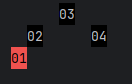
\includegraphics[width=0.25\textwidth]{foutieve_rebuild_n4.png}

\vspace{0.2cm}

Terwijl we perfect 2 rode toppen kunnen krijgen door in bovenstaand voorbeeld de toppen met sleutels 2 en 4 rood kunnen kleuren en die met sleutel 1 kleur 2 kunnen geven zoals volgt:

\vspace{0.2cm}

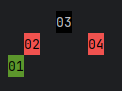
\includegraphics[width=0.25\textwidth]{correcte_rebuild_n4.png}

\vspace{0.2cm}

We moeten dit dus hardcoderen

Gelukkig is dit het enige tegenvoorbeeld, aangezien andere bomen met deze als deelboom de wortel van de deelboom rood hebben gekleurd en je zo toch 2 rode toppen hebt

Zie hier het voorbeeld voor $n = 8$ en $k = 3$:

\vspace{0.2cm}

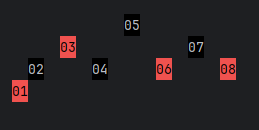
\includegraphics[width=0.5\textwidth]{rainbow_rebuild_n8.png}

\vspace{0.5cm}

\Large (d) tijdscomplexiteit
\vspace{0.3cm}

\large
Het opvragen van de sleutels in gesorteerde volgorde kan in $O(n)$, door deze recursief te doorlopen op dezelfde manier als bij rood-zwart

Dan doen we een aantal berekeningen in $O(1)$ om te zien wat de diepte wordt van onze grootst mogelijke compleet binaire boom

Hierna lopen we over de sleutels en kiezen we degene uit die we zullen gebruiken voor de opbouw van de compleet binaire boom in $O(n)$

Uiteindelijk bouwen we onze compleet binaire boom recursief op in $O(n)$

Het toevoegen van de resterende sleutels kan in $O(n)$, dankzij een bijgehouden lijst, waarbij we de ouders in $O(1)$ kunnen bepalen

Dan overlopen we de rode toppen van onder naar boven en doen we een aantal constante bewerkingen, dit kan dus in $O(n)$

Dus is onze tijdscomplexiteit $O(n)$

\newpage

\Large (e) tijdscomplexiteit voor een reeks van $b$ bewerkingen op een initiëel lege boom
\vspace{0.3cm}

\large
bovengrens toevoegbewerking:

Het maximaal aantal toppen in de boom is $b$, dus een bovengrens is $b * O(k*\log(b)) = O(b * 
 k *\log (b))$

\vspace{0.2cm}

bovengrens opzoekbewerking:

Het maximaal aantal toppen in de boom is $b$, dus een bovengrens is $b * O(k * \log(b)) = O(b * k * \log (b))$

\vspace{0.2cm}

bovengrens verwijderbewerking:

Bij een verwijderbewerking is er meer werk, want de tijdscomplexiteit voor een enkele operatie is $O(k * log(n) + n)$ (indien rebuild zich voordoet)

Maar we kunnen bewijzen dat een bovengrens voor $b$ verwijderbewerkingen $O(b * k * \log(b))$ is:

Gelukkig kan rebuild enkel gebeuren wanneer de helft een grafsteen is en bij elke verwijderoperatie kan er maximum 1 grafsteen bijkomen

Dus komt een rebuild in het slechtste geval voor in een boom met $n$ toppen indien we een startsituatie hadden met $2*n$ toppen en er $n$ verwijderoperaties zijn gebeurd waarbij telkens 1 grafsteen is bijgekomen

Dus voor $n$ zo'n operaties hebben we: $n * O(k * \log (2*n)) + O(n) = O(n * k * \log(n))$

Het maximaal aantal toppen in een boom is $b$, dus voor $b$ verwijderbewerkingen is een bovengrens $O(b * k * \log (b))$
\vspace{0.2cm}

Hierdoor is een bovengrens voor alle bewerkingen $3 * O(b * k * \log (b))$ en dus $O(b * k * \log (b))$

Dit is ook de beste bovengrens, aangezien een reeks bewerkingen bestaat die daaraan voldoet: 

Bv. de sleutels $1 \rightarrow b$ toevoegen, dit levert $\sum_{i=1}^{b} O(\log (i)) = b * O(k *\log (b))$ op

\newpage

\section*{\centering DEEL II: beschrijving implementatie}
\vspace{1cm}

\Large \code{ColouredNode<>}

\vspace{0.3cm}

\large

Deze implementatie van \code{Node} heeft naast de verwachte functies en variabelen nog 3 extra functies:

\vspace{0.2cm}

\code{childrenCount()} en \code{isLeaf()}

Deze functies worden vooral gebruikt bij de verwijderoperatie, om makkelijker de gevallen te onderscheiden, bv. \code{node.isLeaf() \&\& node.getColour() == 1}

\vspace{0.2cm}

\code{toString()}

Deze override was zeer nuttig voor het debuggen

\vspace{0.2cm}

Opvallend is dat ik niet met een \code{parent} variabele heb gewerkt

Deze keuze was bewust gekozen doordat ik een grotere uitdaging wilde

\vspace{0.5cm}

\Large \code{ColouredTree<>}

\vspace{0.3cm}

\large

De abstracte implementatie van \code{SearchTree<>}

\code{RedBlackTree<>} en \code{RainbowTree<>} \textit{extenden} deze klasse

Aangezien een \code{RedBlackTree<>} eigenlijk gewoon een \code{RainbowTree<>} met $k = 2$ is, heb ik veel werk vermeden door een aantal functies of delen van functies in deze klasse te steken

\vspace{0.2cm}

\code{size()} en \code{search()}

Om deze te verwezelijken heb ik al mijn waarden opgeslaan in een \code{HashSet<> values}

Daardoor hoef ik gewoon resp. \code{values.size()} en \code{values.contains()} op te roepen

\vspace{0.2cm}

\code{getSearchPath()}

Deze geeft een lijst met alle nodes op mijn opzoekpad terug

Is zeer nuttig aangezien ik geen \code{parent} variabele heb

\vspace{0.2cm}

\code{add()}

Alle basisgevallen van de twee bomen kan ik samennemen: bestaande sleutel, lege boom, top met corresponderende sleutel is grafsteen, de ouder die niet kleur $k - 1$ heeft

Voor dat laatste geval in een \code{RedBlackTree<>} zet ik zoals al vermeld $k = 2$ en komt dat geval dus voor als de ouder zwart is

Als geen van de gevallen zich voordoet, zoals bv. bij \code{RedBlackTree<>} wanneer de ouder rood is en een top met overeenkomstige sleutel er niet al als grafsteen in zit, dan roep ik de abstracte functie \code{fix2WrongColoursProblem()} op die dit probleem zal afhandelen volgens de implementatie in de twee bomen zelf

\vspace{0.2cm}

\code{remove()}

Het enige basisgeval die ik hierin behandel is wanneer de sleutel nog niet in de boom zit

Indien dit wel het geval is, zoek ik naar de corresponderende top en roep ik de abstracte functie \code{removeSpecialCases()} op

Ik kon nog een aantal andere basisgevallen hierin behandelen, maar dit was een bewuste keuze, omdat ik bij een swap \code{removeSpecialCases()} recursief zal oproepen

\newpage

\code{values()}

Deze bepaal ik recursief:

Eerst de waarden van de recursie van het linkerkind van de wortel, dan die van de wortel zelf en als laatste de recursie van het rechterkind

\vspace{0.2cm}

Er zitten nog een aantal andere functies in deze klasse, maar hierop zal ik later terugkomen

\vspace{0.5cm}

\Large \code{RedBlackTree<>}

\vspace{0.3cm}

\large

\code{fix2WrongColoursProblem()}

We starten met het sorteren van de toppen in een volgorde van boven naar onder, van links naar rechts (de volgorde die ze zullen hebben na de rotering) door gebruik te maken van \code{orderNodes()} uit \code{ColouredTree<>}

Dan bouwen we a.d.h.v. deze sortering onze nieuwe deelboom op

Waarna we op de volgende manier kleuren:

Indien het andere kind van de grootouder voor de opbouw van de deelboom niet rood was, kleuren we de nieuwe wortel zwart en diens kinderen rood

Anders kleuren we de nieuwe wortel rood en diens kinderen zwart

In dat laatste geval zullen we de rotering opnieuw doen als de overgrootouder rood was

Zo blijven we doorgaan tot er geen probleem is of geen overgrootouder is, wat betekent dat we in de wortel zijn aangekomen en we deze gewoon zwart kunnen kleuren

\vspace{0.2cm}

\code{removeSpecialCases()}

Het verwijderen van de wortel indien de boom maar 1 top heeft en het verwijderen van een rood blad kunnen we zonder problemen doen

Het verwijderen van een zwarte top met maar 1 kind wordt waargemaakt met een kleine herbalancering:

Dit kind is zeker rood, anders hadden we geen geldige rood-zwart boom en dus kunnen we dit zwart kleuren en op de plaats van de verwijderde top zetten

Het verwijderen van een zwart blad met een rode ouder is dan weer wat moeilijker:

We weten zeker dat het andere kind van de rode ouder zwart is, anders hadden we geen geldige rood-zwart boom en dus kleuren we de rode ouder zwart en diens kind rood

Indien we nu een probleem hebben veroorzaakt doordat een kind van dat kind rood is, lossen we dit op met \code{fix2WrongColoursProblem()}

Belangrijk is hier dat we niet de geöptimaliseerde kleuring nemen waarbij de kinderen rood zijn, aangezien je dan in de problemen komt als het andere kind van dat kind ook rood is

Het verwijderen van een zwart blad met een zwarte ouder gebeurt simpelweg met een grafsteen die we aanmaken met \code{tombstone()} uit \code{ColouredNode<>}, deze zal van de top een grafsteen maken en indien de helft van de toppen een grafsteen is, \code{rebuild()} oproepen

Indien geen van bovenstaande gevallen past, zitten we zeker met een interne top met 2 kinderen, we zullen aan de hand van \code{swapInternNode()} uit \code{ColouredNode<>} swappen met de top met grootste sleutel uit de linkerdeelboom en \code{removeSpecialCases()} recursief oproepen

Maar let op!

Indien deze swap zou resulteren in het maken van een grafsteen zou onze boom geen zoekboom meer zijn, dus maken we de top grafsteen en swappen we niet

\newpage

\code{rebuild()}

Eerst halen we het aantal toppen en sleutel op via \code{size()} en \code{values()}, om dan de boom leeg te maken

Daarna berekenen we de diepte van de complete binaire boom met $\log(n)$

Indien we niet exact genoeg toppen hebben om een compleet binaire boom te maken zal onze compleet binaire boom 1 niveau kleiner zijn

Dan bereken we de het aantal toppen die we over hebben en halen we die uit de lijst door telkens degene op de even posities van de gesorteerde sleutellijst te nemen totdat we er genoeg hebben

De compleet binaire boom bouwen we dan recursief op met enkel zwarte toppen en hierbij houden we een 2D-lijst bij van de toppen per niveau

Als laatste kunnen we dan de resterende toppen toevoegen als rode bladeren en de optimalisatiestap toepassen, zoals uitgelegd bij theorievraag 1b

\vspace{0.5cm}

\Large \code{RainbowTree<>}

\vspace{0.3cm}

\large

\code{fix2WrongColoursProblem()}

Veel uitleg kan ik hierbij niet geven, de rotering is op dezelfde manier als bij \code{RedBlackTree<>} en de rest werd uitgelegd in theorievraag 2a

\vspace{0.2cm}

\code{removeSpecialCases()}

Het verwijderen van de wortel indien de boom maar 1 top heeft en het verwijderen van een niet-zwart blad kunnen we zonder problemen doen

Het verwijderen van een top met maar 1 kind wordt waargemaakt met een kleine herbalancering:

Dit kind is zeker niet zwart, anders hadden we geen geldige regenboogboom en dus kunnen we dit de oorspronkelijke kleur van de top geven en op de plaats van de top zetten

Het verwijderen van een zwart blad gebeurt op dezelfde manier als bij een zwart blad met zwarte ouder in \code{RedBlackTree<>}

Een interne node wordt ook op dezelfde manier afgehandeld als bij \code{RedBlackTree<>}

\vspace{0.2cm}

\code{rebuild()}

Het geval waarbij $n = 4$ en $k > 2$ werd \textit{gehardcode}

Voor de andere gevallen gebeurt het ophalen van de info, leegmaken van de boom, berekenen van de diepte van de compleet binaire boom en bepalen van de resterende toppen op dezelfde manier als bij \code{RedBlackTree<>}

Bij het opbouwen van de compleet binaire boom wisselen we per rij af met kleur rood en zwart, zoals uitgelegd bij theorievraag 2c

Hierbij houden we een lijst met rode toppen en een lijst met de toppen op het onderste niveau bij

Dan kunnen we de resterende toppen toevoegen als rode bladeren a.d.h.v. de tweede lijst

En als laatste kunnen we over onze lijst met rode toppen gaan en de optimalisatiestap toepassen, wat ook werd uitgelegd in theorievraag 2c

\newpage

\section*{\centering DEEL III: benchmarks}
\vspace{1cm}

Elke benchmark werd 100 keer uitgevoerd, waarvan dan het gemiddelde werd berekend

\vspace{0.5cm}

\Large
1. Voor welke $k$ is mijn regenboogboom het efficiënst?

\large

De benchmarks hiervoor werden uitgevoerd voor $k$ van 2 $\rightarrow$ 1 000 000 voor $n$ = 500 000

\vspace{0.2cm}

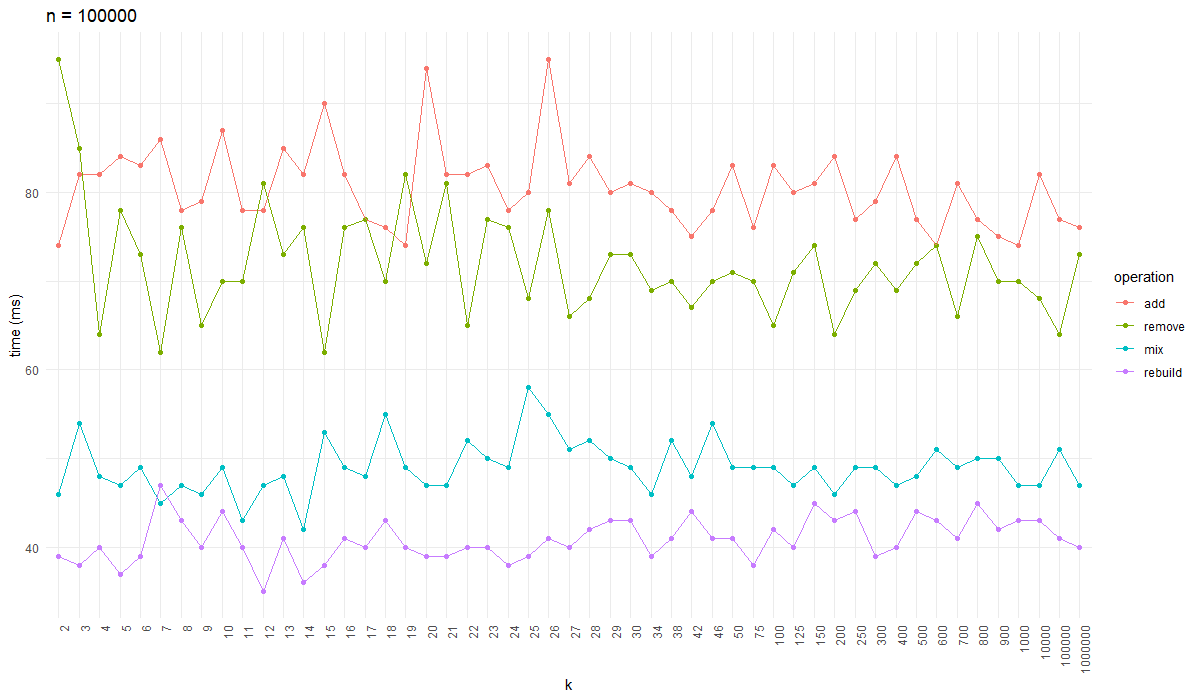
\includegraphics[width=1\textwidth]{benchmark_rainbow.png}

\vspace{0.2cm}

Hieruit kunnen we zien dat de uitvoeringstijden van de operaties voor iedere $k$ ongeveer gelijk zijn

\vspace{0.2cm}

Dit resultaat is zeer interessant:

Hoe groter $k$, hoe groter de maximale diepte, nl. $O(k * \log (n))$, maar ook hoe kleiner het aantal herbalanceringen, want bij het toevoegen duurt het langer vooraleer je aan kleur $k$ - 1 zit en bij het verwijderen zal het geval van niet-zwarte bladeren veel meer voorkomen dan de andere

Tegen mijn initiële verwachtingen in heffen ze elkaar op

Ik dacht namelijk dat de diepte veel zwaarder ging doorwegen dan het aantal herbalanceringen

Maar eigenlijk bij nader inzien is deze opheffing wel logisch

Want door de manier waarop ik mijn herbalanceringen doe, heb je een rood-zwart boom vanboven met de andere kleuren op de laagste niveaus, waardoor je dus met een $O(\log(n) + k)$ diepte zit, wat al veel minder doorweegt dan de maximale diepte

\vspace{0.2cm}

De grotere maximale diepte en kleiner aantal herbalancering zullen elkaar niet exact opheffen

Dus de efficiënste $k$ zal degene zijn waarvoor het verschil in aantal herbalancering het grootst is tegenover het verschil in maximale diepte

De benchmarks werden niet in de perfecte toestand uitgevoerd (schommelend CPU-gebruik, schommelend routerverkeer ...), wat te zien is aan de schommelende resultaten

Dus ik kan enkel een ruime schatting doen voor de efficiënste $k$

Deze schatting levert $k = 9$ op, met een totale tijd van 230 ms voor de 4 operaties

\newpage

\Large
2. Hoe efficiënt is die regenboogboom met optimale $k$ ($k = 9$) in vergelijking met mijn rood-zwart boom?

\vspace{0.2cm}

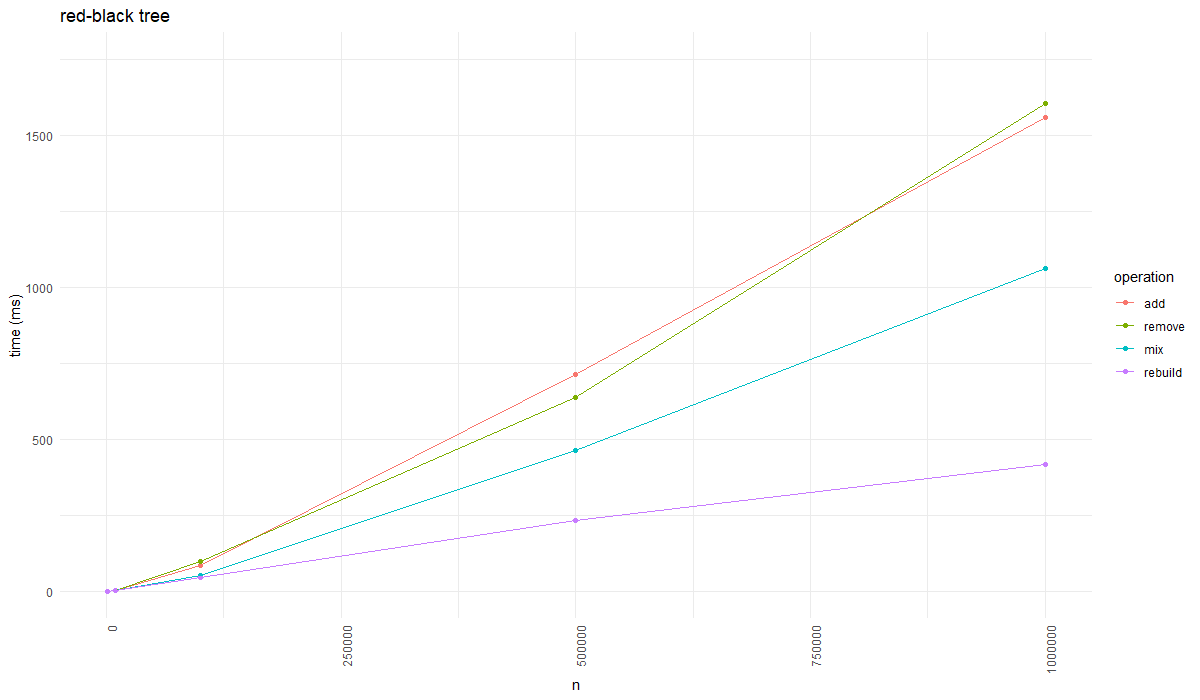
\includegraphics[width=1\textwidth]{benchmark_rainbow_vs_redblack_0.png}

\vspace{0.2cm}

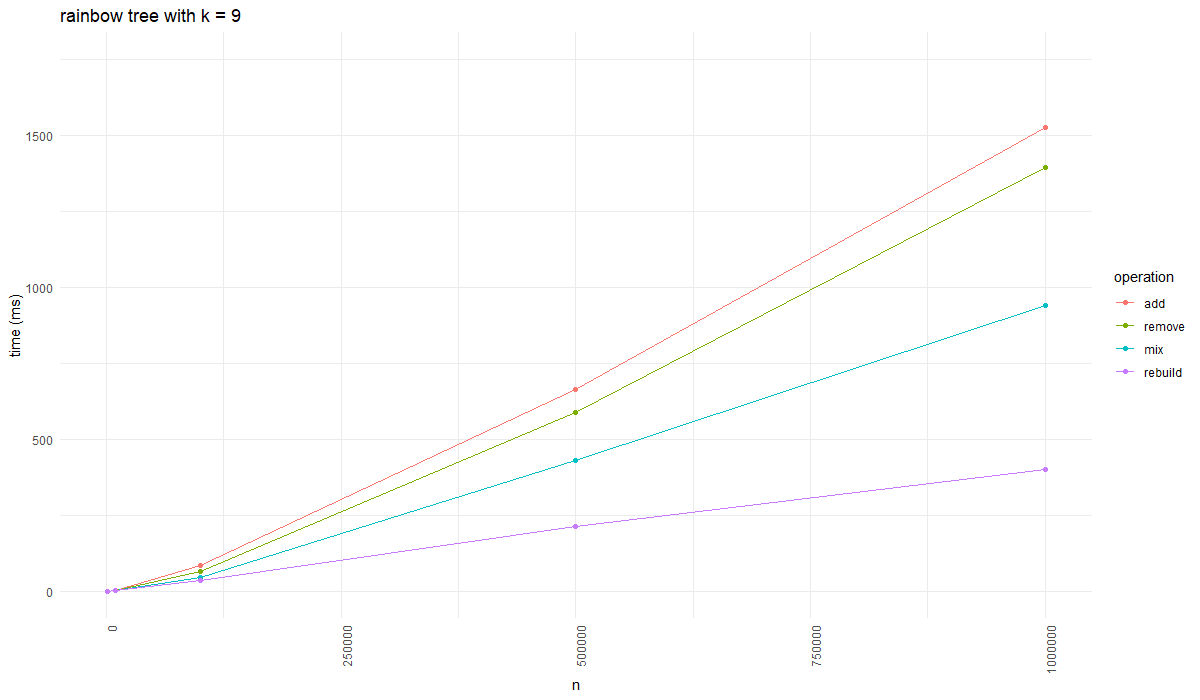
\includegraphics[width=1\textwidth]{benchmark_rainbow_vs_redblack_1.png}

\vspace{0.2cm}

\large

In deze resultaten kunt u zien dat de regenboogboom lichtjes sneller is voor de operaties add, remove en mix

\newpage

Volgens de tijdscomplexiteiten van deze operaties voor beide bomen is dit onlogisch

Maar de manier waarop mijn regenboogboom geïmplementeerd is verklaart dit:

Zoals bij de vorige benchmarks gezegd, zal mijn eigenlijke diepte $O(\log(n) + k)$ zijn en dus voor $k = 9$ zal die $O(\log(n))$ zijn

Dus de diepte's zijn quasi gelijk voor beide bomen

Maar het aantal herbalancering in de regenboogboom is kleiner dan dat in de rood-zwart boom

Het verschil in deze ratio is zo te zien niet gigantisch, maar toch groot genoeg om merkbare verschillen te krijgen

\vspace{0.2cm}

Voor de operatie rebuild zijn de tijden voor beide bomen wel gelijk, wat logisch is, aangezien beide in O(n) gebeuren en eigenlijk het enige mogelijke verschil in tijd, die van de optimalisatiestappen, ook quasi hetzelfde zijn voor beide

\end{document}
